\documentclass[english, 11 pt, class=article, crop=false]{standalone}
\usepackage[T1]{fontenc}
\usepackage[utf8]{luainputenc}
\usepackage{lmodern} % load a font with all the characters
\usepackage{geometry}
\geometry{verbose,paperwidth=16.1 cm, paperheight=24 cm, inner=2.3cm, outer=1.8 cm, bmargin=2cm, tmargin=1.8cm}
\setlength{\parindent}{0bp}
\usepackage{import}
\usepackage[subpreambles=false]{standalone}
\usepackage{amsmath}
\usepackage{amssymb}
\usepackage{esint}
\usepackage{babel}
\usepackage{tabu}
\makeatother
\makeatletter

\usepackage{titlesec}
\usepackage{ragged2e}
\RaggedRight
\raggedbottom
\frenchspacing

% Norwegian names of figures, chapters, parts and content
\addto\captionsenglish{\renewcommand{\figurename}{Figur}}
\makeatletter
\addto\captionsenglish{\renewcommand{\chaptername}{Kapittel}}
\addto\captionsenglish{\renewcommand{\partname}{Del}}

\addto\captionsenglish{\renewcommand{\contentsname}{Innhald}}

\usepackage{graphicx}
\usepackage{float}
\usepackage{subfig}
\usepackage{placeins}
\usepackage{cancel}
\usepackage{framed}
\usepackage{wrapfig}
\usepackage[subfigure]{tocloft}
\usepackage[font=footnotesize]{caption} % Figure caption
\usepackage{bm}
\usepackage[dvipsnames, table]{xcolor}
\definecolor{shadecolor}{rgb}{0.105469, 0.613281, 1}
\colorlet{shadecolor}{Emerald!15} 
\usepackage{icomma}
\makeatother
\usepackage[many]{tcolorbox}
\usepackage{multicol}
\usepackage{stackengine}

% For tabular
\addto\captionsenglish{\renewcommand{\tablename}{Tabell}}
\usepackage{array}
\usepackage{multirow}
\usepackage{longtable} %breakable table

% Ligningsreferanser
\usepackage{mathtools}
\mathtoolsset{showonlyrefs}

% index
\usepackage{imakeidx}
\makeindex[title=Indeks]

%Footnote:
\usepackage[bottom, hang, flushmargin]{footmisc}
\usepackage{perpage} 
\MakePerPage{footnote}
\addtolength{\footnotesep}{2mm}
\renewcommand{\thefootnote}{\arabic{footnote}}
\renewcommand\footnoterule{\rule{\linewidth}{0.4pt}}
\renewcommand{\thempfootnote}{\arabic{mpfootnote}}

%colors
\definecolor{c1}{cmyk}{0,0.5,1,0}
\definecolor{c2}{cmyk}{1,0.25,1,0}
\definecolor{n3}{cmyk}{1,0.,1,0}
\definecolor{neg}{cmyk}{1,0.,0.,0}

% Lister med bokstavar
\usepackage[inline]{enumitem}

\newcounter{rg}
\numberwithin{rg}{chapter}
\newcommand{\reg}[2][]{\begin{tcolorbox}[boxrule=0.3 mm,arc=0mm,colback=blue!3] {\refstepcounter{rg}\phantomsection \large \textbf{\therg \;#1} \vspace{5 pt}}\newline #2  \end{tcolorbox}\vspace{-5pt}}

\newcommand{\regg}[2]{\begin{tcolorbox}[boxrule=0.3 mm,arc=0mm,colback=blue!3] {\large \textbf{#1} \vspace{5 pt}}\newline #2  \end{tcolorbox}\vspace{-5pt}}

\newcommand\alg[1]{\begin{align} #1 \end{align}}

\newcommand\eks[2][]{\begin{tcolorbox}[boxrule=0.3 mm,arc=0mm,enhanced jigsaw,breakable,colback=green!3] {\large \textbf{Eksempel #1} \vspace{5 pt}\\} #2 \end{tcolorbox}\vspace{-5pt} }

\newcommand{\st}[1]{\begin{tcolorbox}[boxrule=0.0 mm,arc=0mm,enhanced jigsaw,breakable,colback=yellow!12]{ #1} \end{tcolorbox}}

\newcommand{\spr}[1]{\begin{tcolorbox}[boxrule=0.3 mm,arc=0mm,enhanced jigsaw,breakable,colback=yellow!7] {\large \textbf{Språkboksen} \vspace{5 pt}\\} #1 \end{tcolorbox}\vspace{-5pt} }

\newcommand{\sym}[1]{\colorbox{blue!15}{#1}}

\newcommand{\info}[2]{\begin{tcolorbox}[boxrule=0.3 mm,arc=0mm,enhanced jigsaw,breakable,colback=cyan!6] {\large \textbf{#1} \vspace{5 pt}\\} #2 \end{tcolorbox}\vspace{-5pt} }

\newcommand\algv[1]{\vspace{-11 pt}\begin{align*} #1 \end{align*}}

\newcommand{\regv}{\vspace{5pt}}
\newcommand{\mer}{\textsl{Merk}: }
\newcommand\vsk{\vspace{11pt}}
\newcommand\vs{\vspace{-11pt}}
\newcommand\vsabc{\vspace{-5pt}}
\newcommand\vsb{\vspace{-16pt}}
\newcommand\sv{\vsk \textbf{Svar:} \vspace{4 pt}\\}
\newcommand\br{\\[5 pt]}
\newcommand{\fpath}[1]{../fig/#1}
\newcommand\algvv[1]{\vs\vs\begin{align*} #1 \end{align*}}
\newcommand{\y}[1]{$ {#1} $}
\newcommand{\os}{\\[5 pt]}
\newcommand{\prbxl}[2]{
	\parbox[l][][l]{#1\linewidth}{#2
}}
\newcommand{\prbxr}[2]{\parbox[r][][l]{#1\linewidth}{
		\setlength{\abovedisplayskip}{5pt}
		\setlength{\belowdisplayskip}{5pt}	
		\setlength{\abovedisplayshortskip}{0pt}
		\setlength{\belowdisplayshortskip}{0pt} 
		\begin{shaded}
			\footnotesize	#2 \end{shaded}}}

\newcommand{\fgbxr}[2]{
	\parbox[r][][l]{#1\linewidth}{#2
}}

\renewcommand{\cfttoctitlefont}{\Large\bfseries}
\setlength{\cftaftertoctitleskip}{0 pt}
\setlength{\cftbeforetoctitleskip}{0 pt}

\newcommand{\bs}{\\[3pt]}
\newcommand{\vn}{\\[6pt]}
\newcommand{\fig}[1]{\begin{figure}
		\centering
		\includegraphics[]{\fpath{#1}}
\end{figure}}


\newcommand{\sectionbreak}{\clearpage} % New page on each section

% Section comment
\newcommand{\rmerk}[1]{
\rule{\linewidth}{1pt}
#1 \\[-4pt]
\rule{\linewidth}{1pt}
}

% Equation comments
\newcommand{\cm}[1]{\llap{\color{blue} #1}}

\newcommand\fork[2]{\begin{tcolorbox}[boxrule=0.3 mm,arc=0mm,enhanced jigsaw,breakable,colback=yellow!7] {\large \textbf{#1 (forklaring)} \vspace{5 pt}\\} #2 \end{tcolorbox}\vspace{-5pt} }


%%% Rule boxes %%%
\newcommand{\gangdestihundre}{Å gonge desimaltall med 10, 100 osv.}
\newcommand{\delmedtihundre}{Deling med 10, 100, 1\,000 osv.}
\newcommand{\ompref}{Omgjering av prefiksar}


%License
\newcommand{\lic}{\textit{Anvend matematikk for grunnskule og VGS by Sindre Sogge Heggen is licensed under CC BY-NC-SA 4.0. To view a copy of this license, visit\\ 
		\net{http://creativecommons.org/licenses/by-nc-sa/4.0/}{http://creativecommons.org/licenses/by-nc-sa/4.0/}}}

%references
\newcommand{\net}[2]{{\color{blue}\href{#1}{#2}}}
\newcommand{\hrs}[2]{\hyperref[#1]{\color{blue}\textsl{#2 \ref*{#1}}}}
\newcommand{\rref}[1]{\hrs{#1}{Regel}}
\newcommand{\refkap}[1]{\hrs{#1}{Kapittel}}
\newcommand{\refsec}[1]{\hrs{#1}{Seksjon}}
\newcommand{\refdsec}[1]{\hrs{#1}{Delseksjon}}

\newcommand{\colr}[1]{{\color{red} #1}}
\newcommand{\colb}[1]{{\color{blue} #1}}
\newcommand{\colo}[1]{{\color{orange} #1}}
\newcommand{\colc}[1]{{\color{cyan} #1}}
\definecolor{projectgreen}{cmyk}{100,0,100,0}
\newcommand{\colg}[1]{{\color{projectgreen} #1}}

\newcommand{\mb}{\net{https://sindrsh.github.io/FirstPrinciplesOfMath/}{MB}}
\newcommand{\enh}[1]{\,\textrm{#1}}

\newcommand{\metode}[2]{
\textsl{#1} \\[-8pt]
\rule{#2}{0.75pt}
}

\newcommand{\linje}{\rule{\linewidth}{1pt} }

% Opg
\newcommand{\abc}[1]{
\begin{enumerate}[label=\alph*),leftmargin=18pt]
#1
\end{enumerate}
}
\newcommand{\abcs}[2]{
	\begin{enumerate}[label=\alph*),start=#1,leftmargin=18pt]
		#2
	\end{enumerate}
}

\newcommand{\abch}[1]{
	\hspace{-2pt}	\begin{enumerate*}[label=\alph*), itemjoin=\hspace{1cm}]
		#1
	\end{enumerate*}
}

\newcommand{\abchs}[2]{
	\hspace{-2pt}	\begin{enumerate*}[label=\alph*), itemjoin=\hspace{1cm}, start=#1]
		#2
	\end{enumerate*}
}

\newcommand{\abcn}[1]{
	\begin{enumerate}[label=\arabic*),leftmargin=20pt]
		#1
	\end{enumerate}
}


\newcommand{\opgt}{
\newpage
\phantomsection \addcontentsline{toc}{section}{Oppgaver} \section*{Oppgaver for kapittel \thechapter}\vs \setcounter{section}{1}}
\newcounter{opg}
\numberwithin{opg}{section}
\newcommand{\op}[1]{\vspace{15pt} \refstepcounter{opg}\large \textbf{\color{blue}\theopg} \vspace{2 pt} \label{#1} \\}
\newcommand{\oprgn}[1]{\vspace{15pt} \refstepcounter{opg}\large \textbf{\color{blue}\theopg\;(regneark)} \vspace{2 pt} \label{#1} \\}
\newcommand{\oppr}[1]{\vspace{15pt} \refstepcounter{opg}\large \textbf{\color{blue}\theopg\;(programmering)} \vspace{2 pt} \label{#1} \\}
\newcommand{\ekspop}{\vsk\textbf{Gruble \thechapter}\vspace{2 pt} \\}
\newcommand{\nes}{\stepcounter{section}
	\setcounter{opg}{0}}
\newcommand{\opr}[1]{\vspace{3pt}\textbf{\ref{#1}}}
\newcommand{\tbs}{\vspace{5pt}}

%Vedlegg
\newcounter{vedl}
\newcommand{\vedlg}[1]{\refstepcounter{vedl}\phantomsection\section*{G.\thevedl\;#1}  \addcontentsline{toc}{section}{G.\thevedl\; #1} }
\newcommand{\nreqvd}{\refstepcounter{vedleq}\tag{\thevedl \thevedleq}}

\newcounter{vedlE}
\newcommand{\vedle}[1]{\refstepcounter{vedlE}\phantomsection\section*{E.\thevedlE\;#1}  \addcontentsline{toc}{section}{E.\thevedlE\; #1} }

\newcounter{opge}
\numberwithin{opge}{part}
\newcommand{\ope}[1]{\vspace{15pt} \refstepcounter{opge}\large \textbf{\color{blue}E\theopge} \vspace{2 pt} \label{#1} \\}

%Excel og GGB:

\newcommand{\g}[1]{\begin{center} {\tt #1} \end{center}}
\newcommand{\gv}[1]{\begin{center} \vspace{-11 pt} {\tt #1}  \end{center}}
\newcommand{\cmds}[2]{{\tt #1}\\[-3pt]
	#2}


\usepackage{datetime2}
\usepackage[]{hyperref}


\begin{document}
\newpage
\section{Indeksregning}
\subsection{Introduksjon}
\parbox{0.6\linewidth}{Innan økonomi er \textit{indeksar} forholdstall som fortel kor mykje størrelsar har forandra seg. For eksempel kosta kroneisen ca 0,75\,kr (!) da den blei lansert i 1953, mens den i 2021 kosta ca 27\,kr. Forholdet mellom prisen i 2053 og i 2021 er da
	\[ \frac{\text{pris 2021}}{\text{pris 1953}}=\frac{27}{0,75}= 36 \]
}
\parbox[r]{0.3\linewidth}{
\includegraphics[scale=2]{kr}}\\[2pt]
I denne samanhengen er talet 36 ein indeks for prisforskjellen på kroneis i 1953 og 2021.

\begin{comment}
	\regv 
	\reg[Indeks]{\vsb
	\[ \frac{\text{verdi 1}}{\text{verdi 2}}\cdot 100 = \text{indeks} \]
	}
	\eks[1]{
	En vare kostet 15\,kr i 2017 og 5\,kr i 1990. Regn ut indeksen for prisendringen fra 2017 til 1990.
	
	\sv 
	Vi deler prisen fra 2017 med prisen fra 1990 og ganger medd 100:
	\[ \frac{15}{5}\cdot 100 = 300 \]
	Indeksen er altså 300.
	}
	\eks[2]{
	En vare kostet i 2000 10 kr. In
	}
\end{comment}
\subsection{Konsumprisindeks og basisår}
\textit{Konsumprisindeksen} (KPI) er ein indeks som skildrar prisnivået på varer og tenester som ein typisk husstand i Norge brukar pengar på i løpet av eit år. Desse varene er \vs

\parbox[t]{0.49\linewidth}{\begin{itemize}
		\item Matvarer og alkoholfrie drikkevarer
		\item Alkoholholdige drikkevarer og tobakk
		\item Klede og skotøy
		\item Bolig, lys og brensel
		\item Møblar, hushaldningsartiklar og vedlikehold av innbo
		\item Helsepleie
\end{itemize}}
\parbox[t]{0.49\linewidth}{\begin{itemize}
		\item Transport
		\item Post- og teletenester
		\item Kultur og fritid
		\item Utdanning
		\item Hotell- og restauranttenester
		\item Andre varer og tenester
\end{itemize}}
For å samanlikne noe må ein alltid ha eit utgangspunkt, og konsumprisindeksen tek utgangspunkt i prisnivået på dei nevnte varene/tenestene i året 2015. 2015 kallast da \textit{basisåret}\footnote{Kva år som er basisår forandrar seg med tiden. Før 2015 blei basisår var 1998 det.}, og i dette året er indeksen satt til 100.\regv
\reg[Basisår]{I eit basisår er verdien til indeksen 100. For konsumprisindeksen er 2015 basisåret.}\vsk

Tabellen under viser samla KPI for dei 10 siste åra:
\begin{center}
	\begin{tabular}{c|c}
		År &  KPI \\ \hline
		2020 & 112,2\\
		2019 & 	110,8\\
		2018 &  112,2 \\
		2017&	105,5\\
		2016&	103,6\\
		2015&	100\\
		2014&	97,9\\
		2013&	95,9\\
		2012&	93,9\\
		2011&	93,3\\
	\end{tabular}
	\captionof{table}{Kunsumprisindeksen for åra 2010-2021. Tal henta frå \net{https://www.ssb.no/priser-og-prisindekser/konsumpriser/statistikk/konsumprisindeksen}{SSB}. \label{KPI}}
\end{center}
Ut ifrå tabellen kan vi for eksempel lese dette:
\begin{itemize}
	\item Da KPI for 2017 er 105,5\,, har prisane stege med 5,5\% sidan 2015.
	\item Da KPI i 2011 er 93,3\,, var prisane 7,7\% lavare i 2011 enn i 2015.
\end{itemize}
\reg[Prosentvis endring frå basisår]{\vs
\[ \text{indeks}-100=\text{prosentvis endring fra basisår} \]
}
\eks[1]{
I juli 2021 var KPI for	matvarer 109,4. Hvor mye har prisen på matvarer endret seg sammenlignet med basisåret?

\sv $ {109,4-100=9,4}  $. Prisen på matvarer har altså økt med 9,4\% sammenlignet med basisåret.
}
\newpage
\eks[2]{
I juli 2021 var KPI for sko 98,0. Hvor mye har prisen på sko endret seg sammenlignet med basisåret?

\sv 
$ 98,0-100=-2 $. Prisen på sko har altså blitt redusert med 2\% sammenlignet med basisåret.  
}
\subsection{Kroneverdi}
Vi har nemnd at en kroneis kosta 0,75\,kr i 1953 og 27\,kr i 2021. Når vi ved to tidspunkt må betale \textsl{forskjellig} pris på den \textsl{same} vara skuldast det ofte at \textit{kroneverdien} har forandra seg;\textsl{ 1\enh{kr} i 1957 var meir verd enn 1\enh{kr} i 2021.
}\vsk

Kroneverdien for eit gitt år reknast ut ifrå KPI til basisåret (100): \regv
	
\reg[Kroneverdi \label{kr}]{\vs
\[ \text{kroneverdi}=\frac{100}{\text{KPI}} \]
{\footnotesize \mer Kroneverdien for basisåret (2015) er 1.}
}
\eks[1]{
KPI i 2012 var 93,9. Rekn ut kroneverdien i 2012.

\sv \vs
\algv{
\text{kroneverdi i 2012} &= \frac{100}{93,9}\\
&\approx 1,06
}
Dette betyr at 1\,kr i 2012 tilsvarar 1,06\enh{kr} i basisåret.
} \vsk

\info{Obs!}{
Ordet \textit{kroneverdi} brukast også når ein samanlikner verdien av 1\enh{kr} opp mot verdien av utenlandsk valuta. Kroneverdi ut ifrå eit basisår og kroneverdi ut ifrå ein valuta er ikkje det same.
}

\reg[Realverdi \label{realverdi}]{
Realverdien til en pengesum er kor mykje ein pengesum ville ha vore verd i basisåret.	
\[ \text{realverdi} = \text{opprinneleg verdi}\cdot \text{kroneverdi} \]
}
\eks{
I 1928 var KPI 3,2 og i 2020 var KPI 112,2. Kva hadde størst realverdi, 10\,000\enh{kr} i 1928 eller 350\,000\enh{kr} i 2020? 

\sv
Vi har at
\algv{
\text{kroneverdi i 1928} &= \frac{100}{3,2}
}
Altså er
\alg{
\text{verdien av 10\,000\enh{kr} fra 1928 i basisår}&= 10\,000\enh{kr}\cdot \frac{100}{3,2} \\
&= 312\,500 \enh{kr}
}
Videre er
\algv{
	\text{kroneverdi i 2012} &= \frac{100}{112,2}
}
Altså er
\alg{
	\text{verdien av 350\,000\enh{kr} fra 1928 i basisår}&= 350\,000\cdot \frac{100}{112,2} \\
	&\approx 311\,943\enh{kr}
}
Altså var 10\,000\enh{kr} meir verd i 1928 enn det 350\,000\enh{kr} var verd i 2020.
}
\subsection{Realløn og nominell lønn}
Kvor god \textit{råd} vi har avheng av kvor mykje vi tener og kva prisnivået er. Tenk at du  hadde ei årsløn på 500\,000\,kr i både 2020 og i 2019. \hyperref[KPI]{\textsl{Tabell \ref*{KPI}}} fortell oss da at du hadde du best råd i 2019, fordi da var prisnivået (KPI) lavare enn i 2020. \vsk

At prisnivået har blitt høgre er det same som at kroneverdien har blitt lavare. Dette betyr igjen at viss løna di var den same i 2019 og 2020, er \textsl{realverdien} til løna din høgre i 2019 enn i 2020. Den opprinnelege løna og realverdien til løna er så mykje brukt i statistikk at dei har fått eigne namn:\regv

\reg[Realløn og nominell løn\label{realnomonn}]{
Nominell løn er løn  mottat eit gitt år. \vsk

Realløna er realverdien til den nominelle løna. 	
}
\eks{
I 2016 tente Per 450\,000 kr, mens i 2012 tente han 420\,000 kr. I 2016 var $ {\text{KPI}=103,6} $, mens i 2012 var $ {\text{KPI}=93,9} $. I kven av desse åra hadde Per best råd?

\sv
For å finne ut kven av åra Per hadde best råd i, sjekkar vi kva år han hadde høgst reallønn\footnote{KPI-verdiene i utrekninga hentar vi frå \hyperref[KPI]{\textsl{Tabell 1}}.} (se \rref{realverdi}):
\alg{
\text{realløn i 2016}&= 450\,000\cdot\frac{100}{103,6}\enh{kr} \\
& \approx 434\,363 \enh{kr}\vn
\text{realløn i 2012}&= 420\,000\cdot\frac{100}{93,9} \\
& \approx 447\,284 \enh{kr}
}
Reallønna til Per var altså høgst i 2012, derfor hadde han betre råd da enn i 2016.
}
\newpage
\reg[Verdi som følger indeks]{
Ein verdi er sagt å ha \textit{fulgt indeks} viss verdi og indeks ved to tidspunkt er like.
\[ \frac{\text{verdi ved tidspunkt 1}}{\text{indeks ved tidspunkt 1}} = \frac{\text{verdi ved tidspunkt 2}}{\text{indeks ved tidspunkt 2}} \]
}

\eks[1]{
	Tabellen under viser ei oversikt over prisen registrert i ein butikk på to varer ved to forskjellige tidspunkt. 
	\begin{center}
		\begin{tabular}{r|r|r|}
			& \textbf{2010} & \textbf{2020}	\\ \hline
			sjokolade & 11,00\enh{kr} & 13,40\enh{kr} \\
			brus	& 12,50\enh{kr} & 19,00\enh{kr}
		\end{tabular}
	\end{center}
I 2010 var KPI 92,1 og i 2020 var KPI 12,2.
Har prisen på nokon av varene fulgt indeks?

\sv

Vi har at
\alg{
\frac{\text{pris på sjokolade i 2010}}{\text{KPI i 2010}} &= \frac{11}{92,1}\approx 0,119 \vn
\frac{\text{pris på sjokolade i 2020}}{\text{KPI i 2020}} &= \frac{13,40}{112,1}\approx 0,119
}
Vidare er
\alg{
	\frac{\text{pris på brus i 2010}}{\text{KPI i 2010}} &= \frac{12,5}{92,1}\approx 0,136 \vn
	\frac{\text{pris på brus i 2020}}{\text{KPI i 2020}} &= \frac{19}{112,1}\approx 0,169
}
Altså er det rimeleg å seie at prisen for sjokolade har fulgt indeks, mens prisen for brus ikkje har gjort det.
}

\section{Lån og sparing}
\subsection{Lån}
Nokre gongar har vi ikkje nok penger til å kjøpe det vi ønsker oss, og må derfor ta opp eit lån frå ein bank. Banken gir oss da ein viss \textit{lånesum} mot at vi betaler tilbake denne, og \textit{renter}, i løpet av ei bestemt tid. Det vanlegaste er at vi undervegs betaler banken det som kallast \textit{terminbeløp}, som på si side består av \textit{avdrag} og renter. Det vi til ei kvar tid skulder banken kallar vi \textit{gjelda}. \vsk

Sei at ein bank låner  oss 100\,000\,kr, som da er lånesummen. Lånet skal vere tilbakebetalt i løpet av 5 år, med eitt terminbeløp kvart år, og renta er 10\%. Det fins forskjellige måtar å betale tilbake eit lån på, men følgande vil som regel gjelde:
\begin{itemize}
	\item \textbf{Summen av alle avdraga skal tilsvare lånesummen}.\os
	 For å gjere det enkelt i vårt eksempel, bestemmer vi oss for å betale tilbake lånet med like avdrag kvart år. Sidan 100\,000 kr skal fordelast likt over 5 år, må det årlege avdraget bli $ \frac{100\,000}{5}\enh{kr}=20\,000 $\,kr.
	\item \textbf{Det ein betaler i avdrag skal trekkast frå gjelda.}\os
	
	Startgjelda er 100\,000\enh{kr}, men det første året betaler vi 20\,000\,kr i avdrag, og da blir gjelda $100\,000\enh{kr}-20\,000\enh{kr} =80\,000\enh{kr} $. Det andre året betaler vi nye 20\,000\,kr, og da blir gjelda $ 80\,000\enh{kr}-20\,000\enh{kr} =60\,000\enh{kr}  $. Og slik fortset det dei neste tre åra.
	\item \textbf{Renter skal reknast av gjelda.}\os 
	Sidan gjelda det første året er 100\,000\,kr, må vi betale \\${ 100\,000\enh{kr}\cdot0,1=10\,000\enh{kr} } $ i renter. Sidan gjelda det andre året er 80\,000\,kr må vi betale ${ 80\,000\enh{kr}\cdot0,1=8\,000\enh{kr} } $ i renter.  Og slik fortset det dei neste tre åra.
	
	\item \textbf{Terminbeløpet er summen av avdraget og rentene}.\os
	
	Av første og tredje punkt får vi at\os
	\centering
	\begin{tabular}{c| c |c}
		 & 1. år & 2. år \\ \hline
		Terminbeløp 
			& $\begin{matrix}
			20\,000\enh{kr} +10\,000\enh{kr}\\
			= \\
			30\,000\enh{kr}
			\end{matrix} $  
				& $\begin{matrix}
					20\,000\enh{kr} +80\,000\enh{kr}\\
					= \\
					28\,000\enh{kr}
					\end{matrix} $ 
	\end{tabular}\os
\raggedright 
Og slik fortset det dei neste tre åra.
\item \textbf{Lånet er fullført når gjelda er lik 0\enh{kr} og alle renter er betalt.}\os
Hvis vi har betalt avdrag lik 20\,000\enh{kr} i 5 år, er gjelda 0\enh{kr}. Har vi da betalt alle rentene også, er lånet fullført. \os

{\footnotesize\mer Du har alltid rett til å betale større avdrag enn det som først er avtalt. Betaler du heile gjelda vil lånet avsluttast så lenge eventuelle renter også er betalt.}
\end{itemize}\vsk
\textbf{Serielån og annuitetslån}\os
To vanlege typer lån er \textit{serielån} og \textit{annuitetslån}. Lånet fra eksempelet vi akkurat har sett på er eit serielån fordi avdraga er like store. Hvis terminbeløpa hadde vore like store, ville det i staden vore eit annuitetslån. Vis lånesum, rente og nedbetalingstid er lik, vil eit serielån alltid medføre minst utgifter totalt sett. For privatpersonar er det likevel veldig populært å velge annuitetslån på grunn av at det er lettare å planlegge økonomien når ein betaler det same beløpet kvar gong. \vsk

\textbf{Kredittkort}\os
\prbxl{0.6}{Kredittkort er eit betalingskort som er slik at viss du f.eks. bruker kortet for å betale 10\,000\,kr, så låner du pengane fra banken. Etter ei tid som er avtalt med banken vil den kreve renter av gjelda din. Til kva tid du betaler denne gjelden er delvis opp til}\qquad
\parbox{0.3\linewidth}{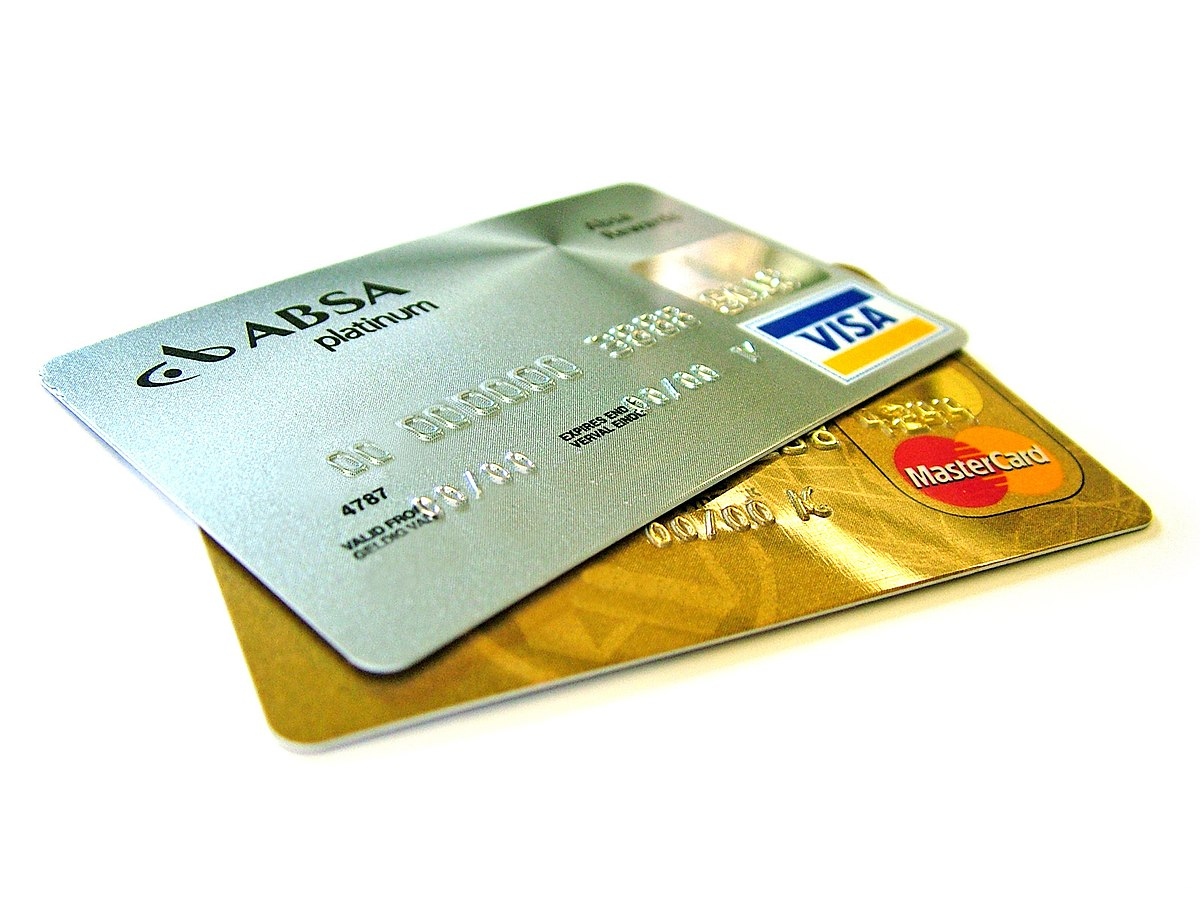
\includegraphics[scale=0.1]{kred}}\\[-2pt]
deg sjølv, men generelt har kredittkort veldig høge renter, så det luraste er å betale før rentekravet har starta!
\regv
\reg[Lån]{
\renewcommand{\arraystretch}{1.5}
\begin{tabular}{>{\bfseries}r l}
	lånesum & Beløpet vi låner av banken. \\
	gjeld & Det vi til ei kvar tid skulder banken. \\
	rente & Prosentandel av gjeld som skal betalast.\\
	avdrag & Det vi betaler ned på gjelda.  \\
	& Summen av avdraga tilsvarer lånesummen.\\
	&ny gjeld $ =  $ gammel gjeld $ - $ avdrag \\
	renter & gjeld $ \cdot $ rente \\
	terminbeløp & avdrag $ + $ renter \\
	serielån & Lån der avdraga er like store. \\
	annuitetslån & Lån der terminbeløpa er like store. \\
	kredittkort & Betalingskort som opprettar eit lån frå banken.
\end{tabular}
}
\newpage
\eks[1]{
Frå ein bank låner du 300\,000\enh{kr} med 3\% årlig rente. Lånet skal betalast tilbake som eit serielån med 5 årlege terminbeløp. \os
\textbf{a)} Kva blir det årlege avdraget?\os
\textbf{b)} Kva er gjelda di etter at du har betalt tredje terminbeløp?\os
\textbf{c)} Kor mye må du betale i renter ved fjerde terminbeløp?\os
\textbf{d)} Kor stort blir det fjerde terminbeløpet?\os 


\sv
\textbf{a)} Sidan 300\,000\,kr skal betalast over 5 år, blir det årlege avdraget
\[ \frac{300\,000\enh{kr}}{5}=60\,000\enh{kr} \]
\textbf{b)} Når tredje terminbeløp er betalt, har du betalt tre avdrag. Det betyr at gjelda di er
\alg{
300\,000-60\,000\cdot3 &= 300\,000-180\,000 \\
&= 120\,000
}
Altså 120\,000\,kr.\os

\textbf{c)} Ut ifrå oppgave b) veit vi at gjelda er 180\,000 kr når fjerde terminbeløp skal betalast. 3\% av gjelda blir da
\[ 180\,000\cdot0,03=5\,400 \]
Altså 5\,400 kr.\os
\textbf{d)} Terminbeløpet tilsvarar avdrag pluss renter. Ut ifrå oppgåve a) og c) veit vi da at det fjerde terminbeløpet blir
\[ 60\,000\enh{kr}+5\,400\enh{kr} =65\,400\enh{kr}\]}
\newpage
\eks[2]{
Frå ein bank låner du 100\,000\,kr med 6,4\% årleg rente. Lånet skal betalast tilbake som eit annuitetslån over 5 år, og banken har da rekna ut at terminbeløpet blir 24\,000\enh{kr}.\os

Rekn ut avdrag og renter for det første terminbeløpet.

\sv
Det første året er gjelda 100\,000\,kr, i renter må du betale 6,4\% av denne:
\[ 100\,000\cdot0,064=6\,400 \]
Altså må du betale 6\,400\,kr i renter det første året.\vsk

Vi har at
\[ \text{terminbeløp}=\text{avdrag}+\text{renter} \]
Dermed er
\[ {\text{avdrag}=\text{terminbeløp}-\text{avdrag}} \]
\[ =24\,000-6400=17\,600 \]
Altså må du betale 17\,600\enh{kr} i avdrag det første året.
}
\newpage
\subsection{Sparing; innskuddsrente og forventa avkastning}
\subsubsection{Innskuddsrente}
Vi har sett at vi må betale renter når vi låner pengar av ein bank, men viss vi i staden sett pengar (gjer eit innskudd) i ein bank  \textsl{får} vi renter: \regv
\reg[Innskuddsrente]{
Innskuddsrente er ei prosentvis auke av pengene du har i banken, gjentatt over faste tidsintervall (månedleg, årleg o.l.) 
}
\eks[1]{
Du sett inn 20\,000\,kr i ein bank som gir 2\% årleg sparerente. Kor mykje pengar har du i banken etter 8 år? 

\sv
For å berekne innskuddsrenter kan vi anvende \rref{progjen}. Sidan renta er 2\%, er vekstfaktoren 1,02. Originalverdien er 20\,000 og antall endringar (tiden) er 8:
\[ 20\,000\cdot1,02^8\approx 23\,433 \]
Du har altså ca. 23\,433\,kr i banken etter 8 år med sparing.
}
\subsubsection{Forventet avkastning}
Ein anna måte å spare pengar på, er å investere i eit aksjefond. Da vil ein snakke om \textit{forventa avkastning}:\regv
\reg[Forventa avkastning]{
Forventa avkastning angir ei \textsl{forventa} prosentvis auke av ei investering, gjentatt over faste tidsintervall.
}
\newpage
\eks[1]{
Du investerer 15\,000 i et aksjefond som forventar 5\% årleg avkastning. Kor mykje er investeringa verd etter 8 år ved ei slik avkastning?

\sv
Også for forventa avkastning kan vi bruke \rref{progjen}. Vekstfaktoren er 1,05, originalverdien er 15\,000 og antall endringar (tiden) er 8:
\[ 15\,000\cdot1,05^8\approx22\,162 \]
Etter 8 år er det forventa at investeringa er verd 22\,162 \enh{kr}.
}
\vsk

\info{Spare med innskuddsrente eller aksjefond?}{
Som regel er forventa avkastning på eit aksjefond høgare enn innskudsrenta du får i en bank, men ulempa er at forventa avkastning ikkje gir nokre garantier. Forventa avkastning oppgir berre auka eksperter antar vil skje. Er du heldig blir auka høgare, er du uheldig blir den lågare, og kan til og med føre til ein \textsl{reduksjon} av investeringa din. I verste fall, rett nok i ekstremt sjeldne tilfeller, kan heile investeringa din ende opp med å bli verd 0\enh{kr}. \vsk

Innskuddsrenten kan også forandre seg noko med tida, men den kan aldri føre til ein reduksjon av investeringen din.
}
\begin{comment}
	\eks[2]{Du betaler 27\,000\,kr med et kreddittkort som krever 1,4\% rente for hver måned du betaler for seint.\os
	
	\textbf{a)} Hvor mye har du i gjeld to år etter for sein betaling?\os
	\textbf{b)} Hva er den årlige renten ved for sein betaling?
	
	\sv
	\textbf{a)} Siden renten er 1,4\%, er vekstfaktoren 1,014. Siden renten er månedlig må vi måle tiden i måneder, og to år er $ {2\cdot12=24} $ måneder. Siden starverdien er 27\,000, får vi:
	\[ 27\,000\cdot1,014^8\approx 37\,649 \]
	Etter to år har du altså ca 37\,649\,kr i gjeld.\os
	
	\textbf{b)} Siden ett år er det samme som 12 måneder blir vekstfaktoren gitt ved: 
	\[ 1,014^{12} \approx1.182\]
	}
\end{comment}


\section{Skatt}
Om du har ei inntekt, må du som regel betale ein del av desse pengane til staten. Desse pengane kallast \textit{skatt} (og nokre gongar \textit{avgift}). Hensikta med skatt er at staten skal ha råd til å gi innbyggerane tilbod som skule, helsetenester og mykje meir. I dag blir blir skatten i stor grad berekna av datasystem, men det er ditt ansvar å sjekke at berekningane er rette $ - $ og da er det viktig å forstå korleis skattesystemet fungerer.\vsk

\info{Obs!}{I eksamensoppgåver og i virkeligheita vil du fort oppdage at skattesystem er presentert på ein litt anna måte enn i denne boka. Dette er blant anna fordi skattereglane kan forandre seg fra år til år, og i denne boka har vi tatt utgangspunkt i skattereglane for 2018. Det viktigaste er ikkje at du husker spesifikt desse reglene, men at du lærer deg kva som meinast med omgrepa \textit{bruttoløn, frådrag, skattegrunnlag, trygdeavgift} og \textit{nettoløn}.}
\subsection{Bruttolønn, frådrag og skattegrunnlag}
\prbxl{0.68}{Dei fleste må betale 23\% av det som kallast \textit{skattegrunnlaget}, som er \textit{bruttolønna} minus \textit{frådrag}. Bruttolønna er lønna du mottek frå arbeidsgiver, mens frådrag kan vere mykje forskjellig. \textit{Personfrådrag} og  \textit{minstefrådrag} er noko alle skattebetalerar får, i tillegg kan ein }\qquad
\prbxr{0.22}{Skattegrunnlag kalles noen ganger \textit{trekkgrunnlag}.} \\[-16pt]

\prbxl{0.66}{blant anna få frådrag viss ein betaler \textit{fagforeningskontigent} eller har gitt pengar til veldedige føremål.}\qquad
\prbxr{0.24}{Fagforeiningskontigent er det du betaler for å være med i ei \net{https://no.wikipedia.org/wiki/Fagforening}{fagforeining}.}\regv

\reg[Bruttoløn, frådrag og skattegrunnlag]{\vs
\begin{center}
	\begin{tabular}{c r}
		\phantom{xxxxx} &bruttolønn	\\
		$ - $ & frådrag \\ \hline
		$ = $ & skattegrunnlag \\ \hline
	\end{tabular}
\end{center}
}
\newpage
\eks{
Bruttoløna til Magnus er 500\,000\,kr. Han får 56\,000\,kr i personfrådrag 97\,600\,kr i minstefrådrag, i tilleg betaler han 1\,000\,kr for årleg medlemskap i fagforeininga \textsl{Tekna}.\os
Kva må Magnus betale hvis han skattar 23\% av skattegrunnlaget?

\sv
Vi startar med å rekne ut skattegrunnlaget, som er bruttoløna minus frådraga:
\begin{center}
	\begin{tabular}{c r l}
	\phantom{xxxxx}	& 500\,000 & bruttolønn	\\
		$ - $& 56\,000 & personfrådrag \\
		$ - $& 97\,600 & minstefrådrag \\
		$ - $& 1\,000 &fagforeningskontigent \\ \hline
		$ = $ &345\,400 & skattegrunnlag \\ \hline
	\end{tabular}
\end{center}
}

\subsection{Trygdeavgift}
Alle lønnsmottakarar må også betale \textit{trygdeavgift}. Dette er ei inntekt staten bruker til å dekke \net{https://no.wikipedia.org/wiki/Folketrygden_(Norge)}{Folketrygda}. Kva ein må betale i trygdeavgift kjem an på kor gammal du er og kva type inntekt du har, men her skal vi berre bry oss om det ein må betale for løn frå ein arbeidsgiver. Da er trygdeavgifta avhengig av alderen: \regv
\reg[Trygdeavgift]{\vs
\begin{center}
	\begin{tabular}{l| r}
		alder & trygdeavgift\\ \hline
		17-69 år &	8,2 \% \\
		under 17 år eller over 69 år &	5,1\%
	\end{tabular}
\end{center}
Trygdeavgifta skal bereknast av bruttoløna.
}
\newpage
\eks{
Jonas og bestemora hans, Line, har begge 150\,000\,kr i løn. Jonas er 18 år og Line er 71 år.\os
\textbf{a)} Kva må Jonas betale i trygdeavgift?\os
\textbf{b)} Kva må Line betale i trygdeavgift?

\sv
\textbf{a)} Sidan Jonas er mellom 17 år og 69 år, skal han betale 8,2\% trygdeavgift:
\[ 150\,000\cdot0,082=12\,300 \]
Altså skal Jonas betale 12\,300\,kr i trygdeavgift.
Sidan Line er over 69 år, skal ho betale 5,1\% trygdeavgift:
\[ 150\,000\cdot0,051=7\,650\]
Altså skal Line betale 7\,650\,kr i trygdeavgift.
}
\subsection{Trinnskatt \label{trinnskatt}}
Av løna di må du også betale ein viss prosent av forskjellege intervall, dette kallast \textit{trinnskatt}:\regv
\reg[Trinnskatt]{\vs
\begin{center}
	\begin{tabular}{l| r |r}
		& Intervall & Skatt \\ \hline
		Trinn 1	& 169 000\,-\,237 900\,kr&	1,4\% \\
		Trinn 2	& 237 900\,-\,598 050\,kr&	3,3\%  \\
		Trinn 3	& 598 050\,-\,962 050\,kr&	12,4\%  \\
		Trinn 4	& Over 962 050\,kr	&15,4\% 
	\end{tabular}
\end{center}
Trinnskatt bereknast av bruttoløna.
}
\newpage
\eks{
Hvis du tener 550\,000 blir utregningen av trinnskatt slik:

\begin{center}
\small
		\begin{tabular}{c|l}
\multirow{3}{*}{Trinn 1} 
\\[-14pt] \hline \\
& Da heile løna er over 237\,900\,kr, må du betale \\
&skatt av  ${(237\,900-169\,000)\enh{kr} = 68\,900\enh{kr}}  $. \os
& Skatt for trinn 1 blir da $ 68\,900\enh{kr}\cdot0,014\approx 965\enh{kr} $.\os \hline \\
\multirow{4}{*}{Trinn 2} 
& Da 550\,000\,kr er over 237\,900\,kr, men under 598\,050\,kr,\\
& må du betale skatt av ${(550\,000-237\,900)\enh{kr} = 312\,100\enh{kr}}  $.  \os
& Skatt for trinn 2 blir da $ 312\,100\enh{kr}\cdot0,033\approx 10\,299\enh{kr} $. \os \hline \\
\multirow{2}{*}{Totalt} 
& Totalt må du betale $ {965\enh{kr}+10\,299\enh{kr}=11\,264\enh{kr}} $\\
& i trinnskatt.
	\end{tabular}
\end{center}
}
\newpage
\subsection{Nettolønn}
Det du sit igjen med etter å ha betalt skatt, trygdeavgift og fagforeiningskontigent kallast \textit{nettoløna}. Med tanke på dei tre tidlegare delseksjonane kan vi sette opp eit reknestykke som dette: \regv
\reg[Nettoløn]{
\begin{center}\vsb
	\begin{tabular}{c r}
	\phantom{xxxxxxx}	& Bruttoløn \\
		$ - $ & Fagforeningskontigent\\ 
		$ - $& 23\% skatt \\
		$ - $ & Trygdeavgift \\
		$ - $ & Trinnskatt \\ \hline
		$ = $ & Nettoløn \\ \hline
	\end{tabular}
\end{center}
}
\eks{
Emblas bruttoløn er 550\,000\,kr. Ho betaler 1500\,kr i året for medlemskap i \textsl{LO} (Norges største fagforeining) og har 409\,900\enh{kr} som skattegrunnlag. Embla er 28 år.\os

Kva er nettoløna til Embla?

\sv \vsb
\begin{center}
	\begin{tabular}{c r l}
		\phantom{xxxxxxx} & 550\,000	& Bruttoløn \\
		$ - $ & 1\,500\, & frådrag for fagforening \\
		$ - $& $ 93\,127 $& 23\% av skattegrunnlaget \\
		$ - $ & 45\,100 & 8,2\% av bruttoløn \\
		$ - $ & 11\,264 & Total skatt for trinn 1 og 2 \\ \hline
		$ = $ & 399\,009& Nettoløn \\ \hline
		
	\end{tabular}
\end{center}
(Den totale trinnskatten har vi henta fra utrekninga i \textsl{Eksempel 1} fra \hyperref[trinnskatt]{\textsl{delseksjon \ref*{trinnskatt}}}.)\vsk

Embla har altså 399\,009\,kr i nettolønn.
}
\section{Budsjett og regnskap}
\subsection{Budsjett \label{budsjett}}
Når ein skal planlegge økonomien sin, kan det vere lurt å sette opp ei oversikt over det ein forventar av inntekter og utgifter. Ei slik oversikt kallast eit \textit{budsjett}. Når ein reknar ut kva inntekter minus utgifter er, finn ein eit \textit{resultat}. Er talet positivt går ein med \textit{overskudd}, er tallet negativt går ein med \textit{underskudd}.

\regv
\eks{
Lisa vil lage ei oversikt over sine månedlege inntekter og utgifter, og kjem fram til dette:
\begin{itemize}
	\item Ho tek på seg kveldsvakter på ein gamleheim. Av dette forventar ho ca. 4\,000\enh{kr} i nettolønn. \\
	\item Ho bruker ca. 4\,500 kr i månaden på mat.
	\item Ho får 4\,360\enh{kr} i borteboarstipend.
	\item Ho bruker ca. 1\,200\enh{kr} på klede, fritidsaktivitetar o.l.
\end{itemize}
Sett opp eit månadsbudsjett for Lisa.

\sv \vsb
\begin{center}
	\begin{tabular}{r r}
		\textbf{Inntekter} & Budsjett \\ \hline 
		løn & 4\,000 \\
		Stipend & 4\,360 \\ \hline
		\textit{Sum} & 8\,360\\\hline 
		& \\
		\textbf{Utgifter} & \\ \hline
		Mat & 4\,500 \\
		Klær, fritid o.l. & 1\,200 \\ \hline
		\textit{Sum} & 5\,700 \\ \hline
		& \\ \hline
		\textbf{Resultat} & 2\,660 \\ \hline
	\end{tabular}
\end{center}
Budsjettet viser at Lisa forventar 2\,660\,kr i overskudd.
}
\newpage
\subsection{Regnskap}
I eit budsjett fører ein opp \textsl{forventa} inntekter og utgifter, mens i eit \textit{reknskap} fører ein opp \textsl{faktiske} innteker og utgifter. Forskjellen mellom budsjett og reknskap kallast \textit{avviket}. For avviket er det vanleg at ein for inntekter og resultat rekner ut '$ {\text{reknskap}-\text{budsjett}} $', mens ein for utgifter rekner ut '$ \text{budsjett}-\text{reknskap} $'. Dette fordi vi ønsker positive tal viss inntekta er større enn forventa, og negative tal viss utgiftene er større enn forventa. \regv
\eks{ I eksempelet fra forrige delseksjon (\ref*{budsjett}) satt vi opp eit månadsbudsjett for Lisa.
	I mars viste det seg at dette blei dei faktiske inntektene og utgiftene hennar:
	\begin{itemize}
		\item Ho fekk ikkje jobba så mykje som ho hadde tenkt. Nettoløna blei 3\,500\,kr.\\
		\item Ho brukte  4\,200 kr i månaden på mat.
		\item Ho fekk 4\,360 i borteboerstipend.
		\item I bursdagsgave fekk ho i alt 2\,000 kr.
		\item Ho brukte ca. 3\,600 på klede, fritidsaktivitetar o.l.
	\end{itemize}
	Sett opp eit reknskap for Lisas mars månad.
	
	\sv \vsb
	\begin{center}
		\begin{tabular}{r r r r}
			\textbf{Inntekter} & Budsjett & Regnskap & Avvik \\ \hline 
			løn & 4\,000 & 3\,500 & $ \color{red} -500 $\\
			Stipend & 4\,360 &  4\,360 &0\\ 
			Bursdagsgave & 0& 2\,000 & 2\,000\\ \hline
			\textit{Sum} & 8\,360 & 9\,860 & 2\,000\\\hline 
			& \\
			\textbf{Utgifter} & \\ \hline
			Mat & 4\,500 & 4\,200 & 300\\
			Klær, fritid o.l. & 1\,200 & 3\,600 & $ \color{red}-2\,400 $\\ \hline
			\textit{Sum} & 5\,700 & 7\,800 & 1\,900\\ \hline
			& \\ \hline
			\textbf{Resultat}  & 2\,660 & 2\,060 & $ \color{red}-600 $ \\ \hline
		\end{tabular}
	\end{center}
Lisa gjekk altså med 2\,060\,kr i overskudd, men 600\,kr mindre enn forventa ut ifrå budsjettet. 	
}

\end{document}